\section{An End-to-End Compression Framework Based
on Convolutional Neural Networks}

\begin{flushleft}
    \author{
    Feng Jiang, 
    Wen Tao, 
    Shaohui Liu, 
    Jie Ren, 
    Xun Guo, 
    Debin Zhao, 
    \emph{Member, IEEE}
    }
\end{flushleft}

\begin{center}
    \emph{IEEE TRANSACTIONS ON CIRCUIT AND SYSTEMS FOR VIDEO THECNOLOGY, VOL. 28, NO. 11, OCTOBER 2018}
\end{center}

\subsection{INTRODUCTION}
In recent years, within the field of computer vision, remarkable results have 
been achieved with regard to image compression. The purpose of compression 
is to be able to transmit, or save, the entire image at low bit rates. As far as 
decompression is concerned, deblocking and denoising techniques have been 
developed that are useful for obtaining good images. Further pre-processing 
steps have been found to negatively impact in system performance. Therefore 
the proposed method uses a framework composed of two convolutional 
networks (\emph{CNNs}). The first network, called compact convolutional neural 
newtork (\emph{comCNN}), is used for compression and uses the JPEG, JPEG2000 
and BPG encoding codecs. The second network, called reconstruction convolutional 
neural network (\emph{RecCNN}), is used for image decompression. A 
first example of the work carried out by the proposed framework is visible in 
the Fig. \ref{fig:output}.
\begin{figure}[h!]
    \centering
    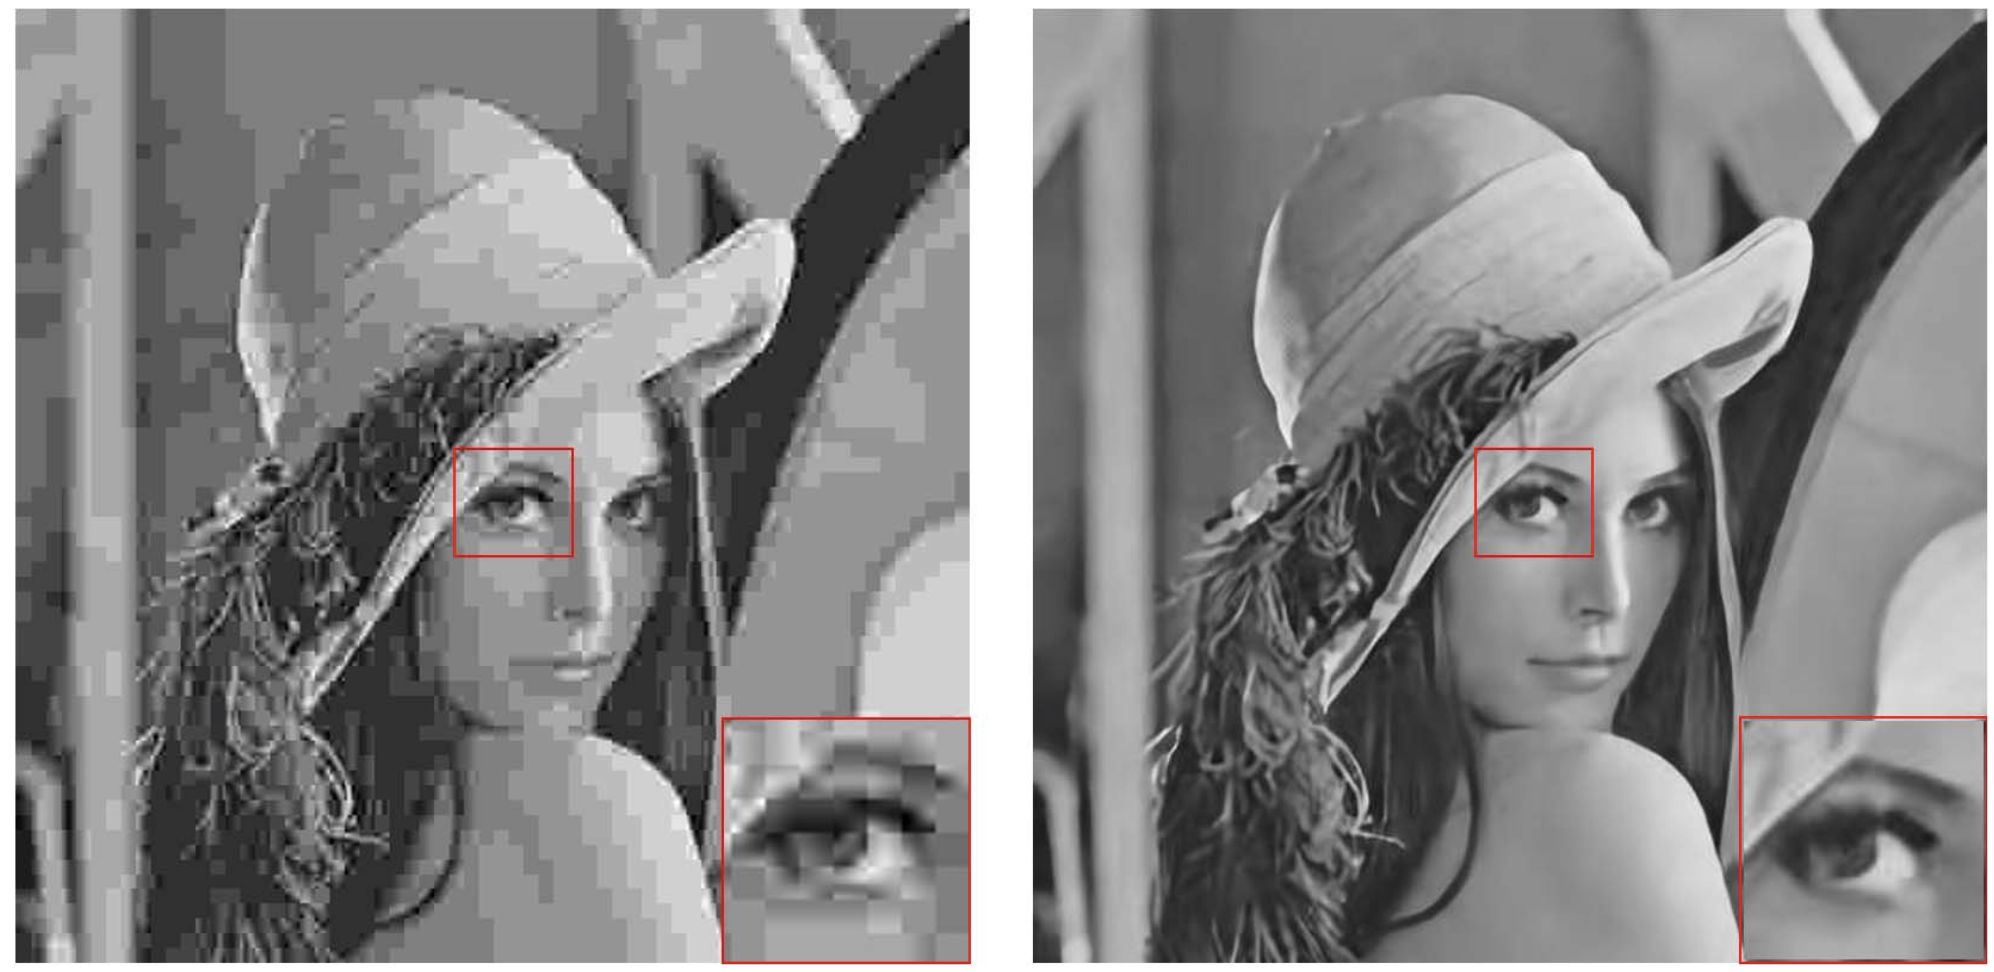
\includegraphics[width = 0.6 \linewidth]{images/paper3/output .png}
    \centering
    \caption{Left: the JPEG-coded image. Right: the decoded image.}
    \label{fig:output}
\end{figure}

\subsection{RELATED WORK}
\subsubsection{Image Deblocking and Artifacts Reduction}
Going back to talking about the deblocking technique, this is useful for removing 
all those blocks that visually worsen the appearance of each image. 
The various restoration techniques model the distortion created in the compression 
phase in order to reduce artifacts. Many methods already proposed 
in the state of the art use techniques that have a great impact on performance 
when they adopt iterative restoration processes. Therefore, the proposed 
method tries to obtain the same result but with a lower computational 
cost.

\subsubsection{Image Super-Resolution Based on Deep Learning}
Convolutional neural networks (\emph{CNNs}) have been used for super resolution 
(\emph{SR}) images especially when residual learning and gradient-based optimization 
algorithms have been proposed to train a deep network. According to 
some studies, the depth of a network doesn't always lead to good performance. 
Other researchers, on the other hand, claim the opposite.

\subsubsection{Image Compression Based on Deep Learning}
Deep learning was used for lossy and loseless compressions achieving good 
performance. There have been some methods that have prevailed over others. 
However, all of these methods ignore compatibility with various image codecs, 
thus limiting their use in some existing systems. The proposed framework 
solves this problem by operating with different image codecs, also taking into 
account the compression performance.